\section{Quantifier Elimination with the Virtual Substitution}
\label{sec:quantifier-elimination-with-the-virtual-substitution}
Let $\varphi^\mathbb{R}$ is a quantifier-free real-arithmetic formula where $x\in \varphi^\mathbb{R}$ and $x$ has at most degree $2$ in $\varphi^\mathbb{R}$. After eliminating existential and universal qualifier with virtual substitution we will get the following equivalences,
\begin{alignat}{2}
	&\exists x. \varphi^\mathbb{R} \Longleftrightarrow \bigvee\limits_{t\in T(x,\varphi^\mathbb{R})}  (\varphi^\mathbb{R} [t\backslash\backslash x] \wedge C_t)\qquad   \\
	& \forall x. \varphi^\mathbb{R} \Longleftrightarrow \bigwedge\limits_{t\in T(x,\varphi^\mathbb{R})}  (C_{t}\rightarrow\varphi^\mathbb{R} [t\backslash\backslash x] )\qquad
\end{alignat}

Now, let us consider $\exists x.\varphi$ where, $\varphi = (x^{2}y + x + y = 0) \wedge (y^{2} -2 < 0)$. We already constructed all the test candidates for $x$ and $y$. Also we get to know about substitution rules with virtual substitution. By using the substitution rules, we eliminate all occurrences of $x$ and $y$ from $\varphi$. Then we get the following equivalence holds.
$$ \exists x\exists y. \varphi \Longleftrightarrow \bigvee\limits_{t_{1}\in T(x,\varphi)}(\bigvee\limits_{t\in T(y,\varphi^{\prime})}  (\varphi^{\prime} [t_{2}\backslash\backslash y] \wedge C_{t_{2}}))$$
where, $\varphi^{\prime} = (\varphi [t_{1}\backslash\backslash x] \wedge C_{t_{1}})$.
\begin{center}
	\begin{figure}[htb]
\definecolor{ffvvqq}{rgb}{0.44313725490196076,0.44313725490196076,0.44313725490196076}
\definecolor{qqqqff}{rgb}{0.3333333333333333,0.3333333333333333,0.3333333333333333}
\begin{tikzpicture}
	[line cap=round,line join=round,>=triangle 45,x=2.2239498017171777cm,y=1.4852526944330273cm]
	\draw[->,color=black] (-3.1381482009239074,0.) -- (3.6066083526718855,0.);
	\foreach \x in {-3.,-2.5,-2.,-1.5,-1.,-0.5,0.5,1.,1.5,2.,2.5,3.,3.5}
	\draw[shift={(\x,0)},color=black] (0pt,2pt) -- (0pt,-2pt);
	\draw[->,color=black] (0.,-2.134493672850494) -- (0.,1.2319368468454657);
	\foreach \y in {-2.,-1.5,-1.,-0.5,0.5,1.}
	\draw[shift={(0,\y)},color=black] (2pt,0pt) -- (-2pt,0pt);
	\clip(-3.1381482009239074,-2.134493672850494) rectangle (3.6066083526718855,1.2319368468454657);
	\draw[line width=1.2pt,color=qqqqff,smooth,samples=100,domain=-3.1381482009239074:3.6066083526718855] plot(\x,{(\x)^(2.0)-2.0});
	\draw[line width=1.2pt,color=ffvvqq,smooth,samples=100,domain=-3.1381482009239074:3.6066083526718855] plot(\x,{1.0-4.0*(\x)^(2.0)});
	\begin{scriptsize}
	\draw[color=black] (-1.3965672407894814,0.7888289427512096) node {$y^{2}-2$};
	\draw[color=black] (-1.05,-1.6854380116543015) node {$1-4y^{2}$};
	\draw [color=black] (-0.5,0.)-- ++(-2.5pt,-2.5pt) -- ++(5.0pt,5.0pt) ++(-5.0pt,0) -- ++(5.0pt,-5.0pt);
	\draw[color=black] (-0.6222469468048416,0.1881054754556408) node {$\frac{-1}{2}$};
	\draw [fill=black] (-1.4142135623730951,0.) circle (1.5pt);
	\draw[color=black] (-1.626306026299163,-0.13307340804892073) node {$-\sqrt{2}$};
	\draw [color=black] (0.5,0.)-- ++(-2.5pt,-2.5pt) -- ++(5.0pt,5.0pt) ++(-5.0pt,0) -- ++(5.0pt,-5.0pt);
	\draw[color=black] (0.6029910161940414,0.19405323255757712) node {$\frac{1}{2}$};
	\draw [fill=black] (1.4142135623730951,0.) circle (1.5pt);
	\draw[color=black] (1.3167218684264004,0.11673239023240492) node {$\sqrt{2}$};
	\draw [fill=black] (-1.3121867706294554,0.) circle (1.5pt);
	\draw[color=black] (-1.1397018146733018,0.15241893284402286) node {$-\sqrt{2}+\epsilon$};
	\draw [color=black] (0.06769287701977207,0.)-- ++(-2.5pt,-2.5pt) -- ++(5.0pt,5.0pt) ++(-5.0pt,0) -- ++(5.0pt,-5.0pt);
	\draw[color=black] (0.15690923354881695,0.15241893284402286) node {$0 + \epsilon$};
	\draw [fill=black] (1.5,0.) circle (1.5pt);
	\draw[color=black] (1.6319529948290257,-0.1271256509469844) node {$\sqrt{2} + \epsilon$};
	\end{scriptsize}
\end{tikzpicture}
\caption{Solution of $y$ in $\varphi_{4}$ where $x = x_{0}$ and $x_{2}$}
\label{fig:graph}
\end{figure}
\end{center}
The solutions of $x$ and $y$ for $\varphi$ is shown in the figure 2 and 3. Also we can have an overview of virtual substitution though figure 4.
\begin{figure}[htb] % where to insert the figure: h=here, t=top, b=bottom,
	% the order htb shows which position is preffered
	\begin{center}
	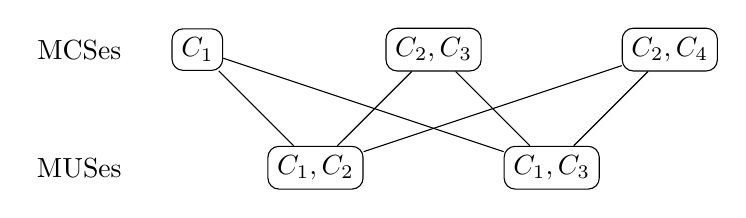
\begin{tikzpicture}[scale=1.5, 
				    state/.style={draw, rounded corners, fill=none,
				    			  text centered, text=black}]
	\node[] (u0) at (1, 2) {MCSes};
	\node[state] (u1) at (2, 2) {$C_{1}$};
	\node[state] (u2) at (4, 2) {$C_{2}, C_{3}$};
	\node[state] (u3) at (6, 2) {$C_{2}, C_{4}$};
	\node[state] (u4) at (3, 1) {$C_{1}, C_{2}$};
	\node[state] (u5) at (5, 1) {$C_{1}, C_{3}$};
	\node[] (u6) at (1, 1) {MUSes};
	
	\path[-] 	(u1)  edge   (u4);
	\path[-] 	(u1)  edge   (u5);
	\path[-] 	(u2)  edge   (u4);
	\path[-] 	(u2)  edge   (u5);
	\path[-] 	(u3)  edge   (u4);
	\path[-] 	(u3)  edge   (u5);

\end{tikzpicture}

	\end{center}
	\caption{Example of Virtual Substitution.}
	\label{fig:graph}
\end{figure}

We get the proof of equation (4.1) which is explained on the above by an example. Equation (4.2) can be implied by equation (4.1) as follows.
%C_{\sim}(\varphi^\mathbb{R})=C_{\sim}(\neg\varphi^\mathbb{R})
\begin{alignat}{2}
	& \forall x. \varphi^\mathbb{R}\qquad   
	&&\stackrel{}{\Longleftrightarrow} \neg\exists x.\neg\varphi^\mathbb{R} \\
	& 
	&&\stackrel{4.1}{\Longleftrightarrow} \neg(\bigvee\limits_{t\in T(x,\varphi^\mathbb{R})}) \neg(\varphi^\mathbb{R} [t\backslash\backslash x] \wedge C_t) \\
	& 
	&&\stackrel{}{\Longleftrightarrow} \bigwedge\limits_{t\in T(x,\neg \varphi^\mathbb{R})} (\varphi^\mathbb{R} [t\backslash\backslash x] \vee\neg C_{t}) \\
	& 
	&&\stackrel{}{\Longleftrightarrow}  \bigwedge\limits_{t\in T(x, \varphi^\mathbb{R})} (C_{t} \rightarrow \varphi^\mathbb{R} [t\backslash\backslash x])
\end{alignat}
